The rationale of this section is to present the use case scenario (the one we call hereinafter Melano Sorter) that will be used throughout the document as the roadway lines to explain concepts and adopted solutions.
The use case describes the hob handling and palletizing operations carried out by within the Melano production plant in Italy (Whirlpool). The elements characterizing this use case scenario from the simulation viewpoint are reported below:

\begin{itemize}
\item In the plant situated in Melano Whirlpool produces over a hundred different configurations of cooking hobs, belonging to three categories: gas, electric or pyro-ceramic. The production is organized in batches;  hobs the same type are aggregated taking into account different orders. Each batch (and every hob in it)  is identified by a code to ensure a high level of traceability. For the same reason, as soon as a single hob is released, an automated reading system records its associated event and communicates it in real-time to the ERP. 
\item The cooking hobs are realized by 14 production stations; each station produces one hob at a time and it is specialized in producing items of only one category (gas, electric, pyro-ceramic).  The automation of the production lines is achieved by means PLCs connected to a MES. Seven palletizers are placed at the end of the stations; they have the task of aggregating in a pallet (generally) 6 elements belonging to the same lot and assigning a unique 2D barcode to the pallet. Small differences in lot size are to be ascribed to the quality control process (affecting about 2\% of items produced). The pallets are then taken over by a raised conveyor of about 1 kilometer long. The length of the conveyor, its average speed as well as the shelf life of the pallets on it are known data of the problem. 
\item On the end of the conveyor there is a 2D barcode reader and a PLC-based automation system, which we refer to hereinafter with the term "Sorter". The sorter has the task of assigning the pallets out of the conveyor to different shipping lines. The barcode reader is placed between the end of the conveyor and the sorter. In this way the sorter becomes aware of the particular type of product contained in the pallet and can decide on which output line (also referred to as “Bay”) to allocate it. The sorter, at the beginning of the earliest shift, assigning each available bay to a particular type of hob. Moreover, depending on the particular production plan, a particular hob type can be assigned to more than one bay. Please notice that, until the next day the hob type/shipping line configuration cannot be modified. 
\item The Melano Whirlpool plant features 18 shipping lines (bays) freely assignable to any type of product. There is also a further bay, which will be indicated by the phrase "mixed bay" to which the sorter directs all those pallets that can not be assigned to regular bays. Finally, there is a bay for incomplete pallets. Regular bays are handled through a forklift that picks up pallets and places them in the corresponding area of the warehouse, whereas the  mixed and incomplete bays pallets are handled manually.
\end{itemize}
	
Figure~\ref{fig:sorter1} below shows schematically the "Sorter" sub-system of the Melano plant.
In the vision of the FAR-EDGE project, Whirlpool will benefit from modeling and simulation of this use case as it will be possible to evaluate different layout configurations and operating logics for the "sorter" without actually stopping the production and implementing the changes. Therefore, working in partnership with WP6, we will act in two successive phases:
\begin{itemize}
\item In the first phase we will create a simulation model (to be run in a Discrete Events Simulator – DES) capable of faithfully representing the current configuration of Melano site. To do this we will analyze the data that Whirlpool will make available to the consortium; to assess the suitability of the model to represent the status quo, we will compare the KPI values obtained through simulation with those measured in the field. This work will be done mainly within the WP4.
\item In the second phase, a what-if analysis will be carried out using alternative simulation scenarios in which the layout (for example, the number of shipping bays) or the algorithm implemented within the "sorter" will be changed. The goal of this phase is to identify margins of improvement with respect to the current situation. This second phase will focus on WP6. Example of questions to be answered in the what-if analysis are:
\begin{itemize}
\item In case of a capacity increase, will the sorter able to manage the normal flow?
\item In case of production plan changes; will the sorter able to manage the normal flow? 
\item In case of production mix changes; will the sorter able to manage the normal flow? 
\item In case of physical reconfigurations, will the sorter able to manage the normal flow? 
\end{itemize}
\end{itemize}


As for T4.1, and specifically this document, this use case scenario has been select among the others for its simplicity; therefore, it can be easily used to explain the various elements of the FAR-EDGE CPS data model and the transformation rules from our from internal model to other formats like JSON.

\begin{figure}
	\centering
	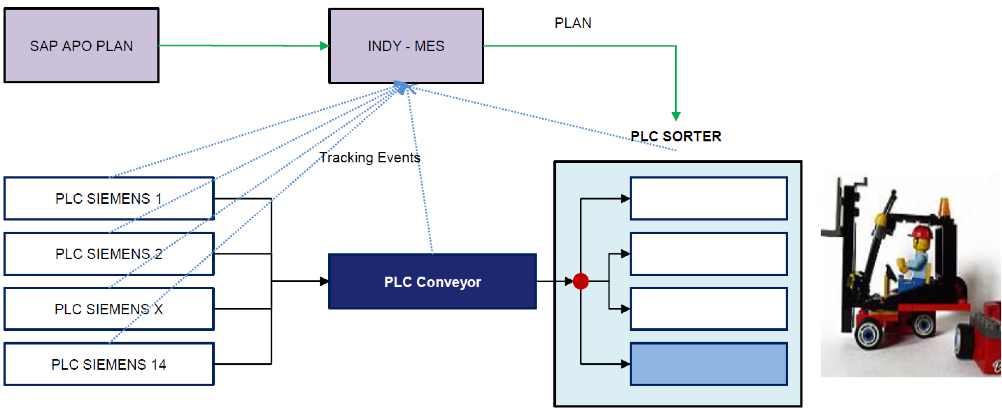
\includegraphics[width=\linewidth]{images/Melano1}
	\caption{Melano sorter use case scenario}
	\label{fig:sorter1}
\end{figure}

